\chapter{Testy systemu}
Rozdział szósty opisuje testy przeprowadzone dla stworzonego systemu repozytorium testów. Celem testów jest weryfikacja poprawnego działania systemu i dowiedzenia spełnienia założonych funkcjonalności. W tym celu zostało określone środowisko testowe na którym wykonano zdefiniowaną pulę testów.

\section{Definicja środowiska testowego}

Weryfikacja aplikacji powstałej jako wynik niniejszej pracy dokonana została poprzez weryfikacje funkcjonalności aplikacji względem przykładowego cyklu życia systemu. Stworzona została charakterystyka systemu, który w pełni może wykorzystać możliwości aplikacji. Następnie stworzone zostały scenariusze, które przeglądowo przechodzą przez możliwe kroki podczas specyfikacji i wykonania fazy testowania oprogramowania.

Specyfikowany system jest systemem zarządzania magazynem o roboczej nazwie \textit{magar}, w którego skład wchodzą następujące produkty:
\begin{enumerate}
  \item interfejs skanujący kody kreskowe produktów -- nazwa robocza \textbf{kodex};
  \item część administracyjna do definiowania i dodawania produktów -- nazwa robocza \textbf{backadm};
  \item część statystyczna prezentująca w sposób graficzny dane zebranie w systemie -- nazwa robocza \textbf{statos}.
\end{enumerate}

Produkt \textit{kodex} pośredniczy pomiędzy urządzeniami końcowymi czyli skanerami kodów kreskowych a scentralizowaną bazą danych. Założeniem jest możliwość obsługi trzech różnych skanerów kodów kreskowych:
\begin{itemize}
  \item skaner1 i skaner2 wyprodukowany przez firmę A,
  \item skaner3 wyprodukowany przez firmę B.
\end{itemize}
Skaner1 i skaner2 posiadają wspólny interfejs konfiguracyjny i podłączane są do systemu za pomocą kabli typu A. Skaner3 posiada natomiast inny sposób konfiguracji i podłączany jest za pomocą kabli typu B.

\section{Scenariusz 1: tworzenie bazy testów}
Scenariusz pierwszy polega na stworzeniu trzech różnych grup testów i 6 przypadków testowych. Przynajmniej jeden przypadek testowy powinien korzystać z funkcjonalności tworzenia warunku w zależności od wyboru urządzeń końcowych. W przypadku systemu magur składowe testów warunkowane są użyciem produktów pochodzących od dostawcy A lub od dostawcy B.

Zdecydowano się na utworzenie następującej hierarchii grup testowych (rezultat widoczny po prawej):


\begin{tabular}{l l}
\begin{minipage}{0.5\textwidth}
\begin{itemize}
    \item testy funkcjonalne,
    \begin{itemize}
      \item część administracyjna,
      \item część statystyczna  ,    
    \end{itemize}
    \item testy niefunkcjonalne.
  \end{itemize}
\end{minipage}
&
\begin{minipage}{0.5\textwidth}
              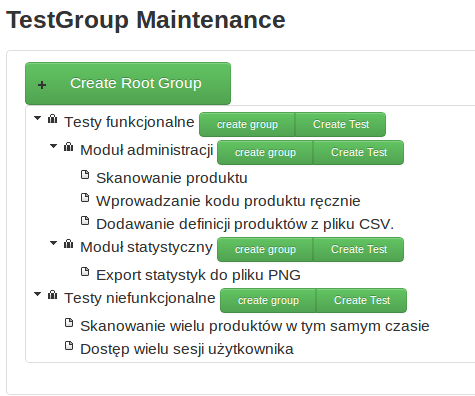
\includegraphics[width=\linewidth]{img/screen/listaTestow.png}            
          
\end{minipage}

\end{tabular}

  
  
  Podczas tworzenia definicji testów, sprawdzona została możliwość dodawania elementów, których włączenie w finalną postać testu jest ograniczona spełnieniem warunku. Przykładem takiego elementu jest dodanie warunku początkowego jakim jest konfiguracja skanera przed przystąpieniem do testowania. Skanery pochodzące od różnych producentów posiadają inny interfejs tak więc wszystkie testy wymagające wstępnego ustawienia interfejsu wymagają dodania dwóch rozdzielnych stanów początkowych przy czym tylko jeden ze stanów włączany zostaje do końcowej definicji testu.
   \begin{figure}[h]
  \begin{center}
    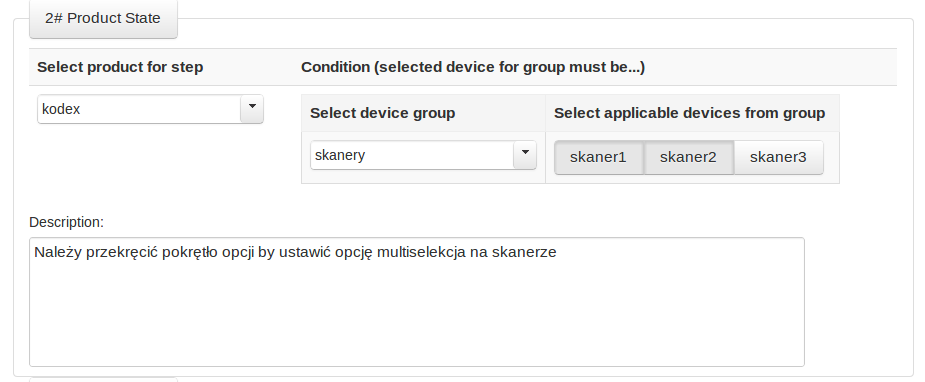
\includegraphics[scale=0.4]{img/screen/stanProdutuZwyboremWarunku.png}
    \label{fig:stanProduktuZwarunkiem}
    \caption{Stan produktu ze zdefiniowanym warunkiem}
  \end{center}
\end{figure}
\pagebreak

Po zakończeniu definiowania testu, wystem wyświetla ekran podsumowujący prezentujący definicje poszczególnych elementów testu wraz z warunkami (Rysunek \ref{fig:podsumowanieTestu}).

  \begin{figure}[h]
  \begin{center}
    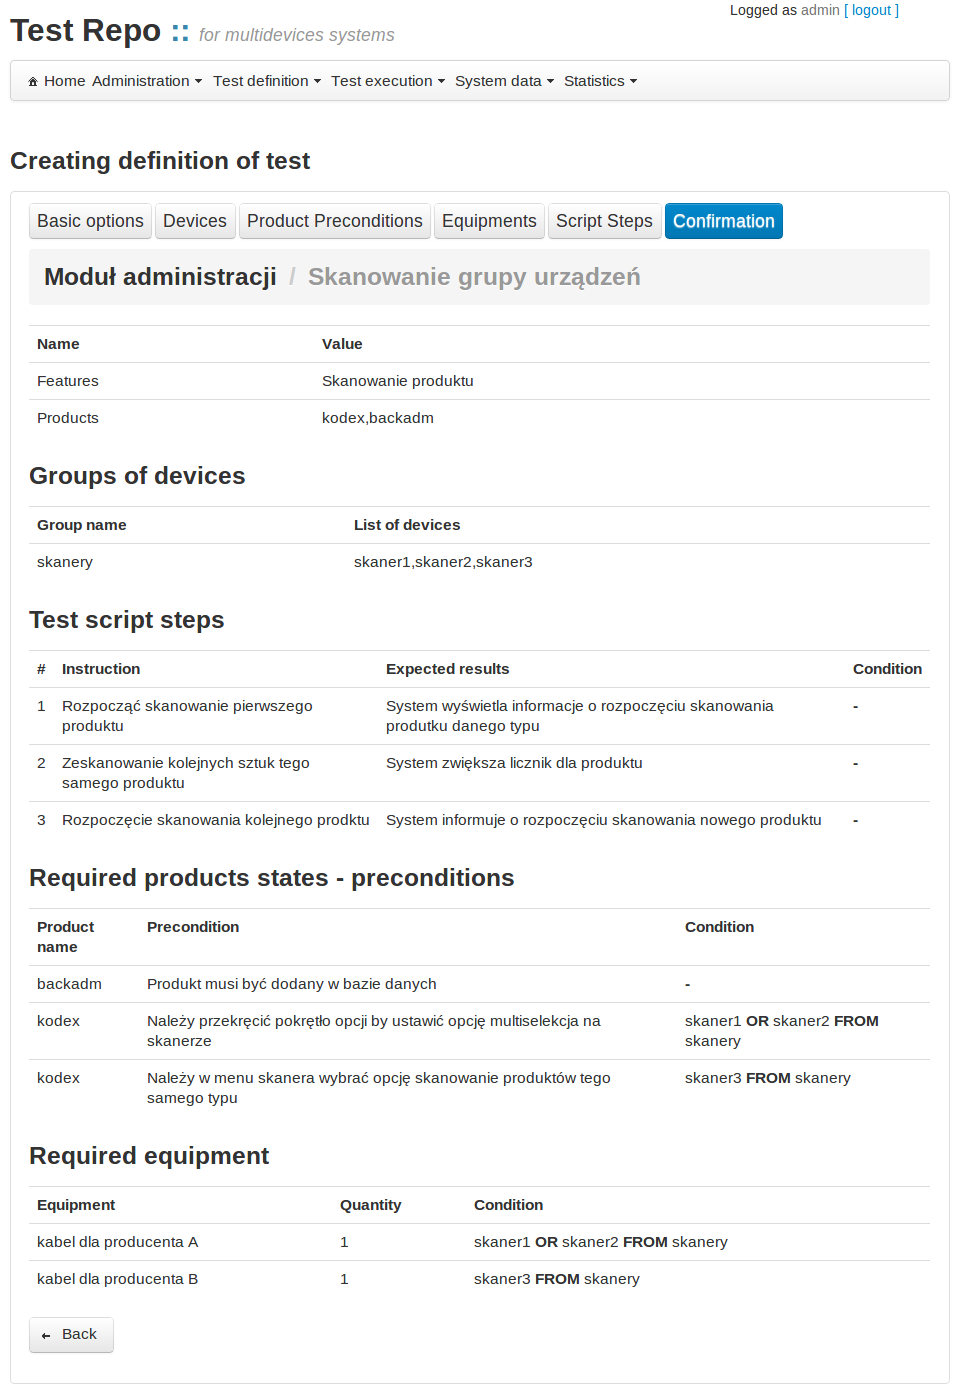
\includegraphics[scale=0.4]{img/screen/tworzenieTestuPodsumowanie.png}
    \caption{Podsumowanie definicji testu}
    \label{fig:podsumowanieTestu}
  \end{center}
\end{figure}

\section{Scenariusz 2: tworzenie planu testów}

Scenariusz drugi zakłada stworzenie dwóch planów testowych, w których skład wchodzą testy tego samego typu. Plan testowy pierwszy zakłada iż testowane są jedynie urządzenia końcowe od dostawcy A, natomiast założeniem drugiego planu testowego jest wykorzystanie urządzeń końcowych pochodzących od dostawcy B.

Stworzenie dwóch planów testowych dla rozłącznych typów urządzeń skutkuje wyprodukowaniem innej końcowej definicji testów do wykonania. Różnice wynikają w doborze dla testów istniejących w poszczególnych planach jedynie tych elementów składowych, które spełniają warunki dla urządzeń końcowych.

Ostatnim krokiem podczas tworzenia nowego planu testów jest określenie urządzeń końcowych dla testów wchodzących w skład testu. Wyboru dokonuje się poprzez wybór dla każdego z testów jednego urządzenia dla każdej ze zdefiniowanych grup urządzeń.

  \begin{figure}[h]
  \begin{center}
    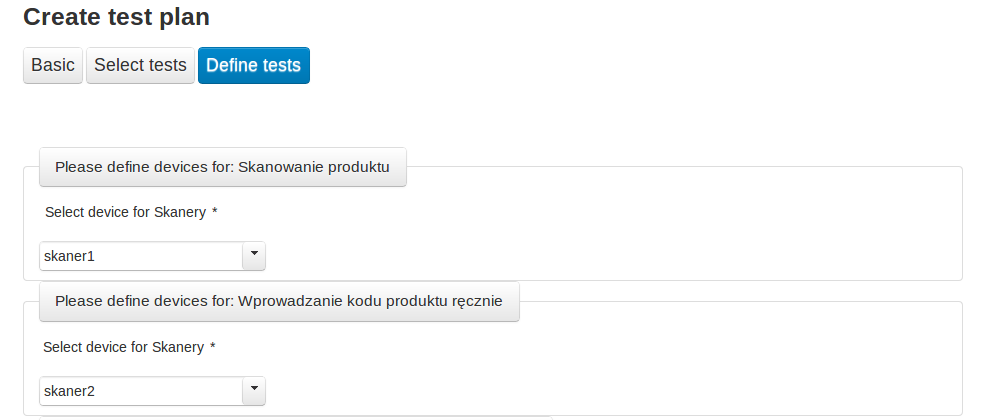
\includegraphics[scale=0.4]{img/screen/tworzeniePlanuWyborUrzadzen.png}
    \caption{Wybór urządzeń końcowych dla planu testowego}
    \label{fig:wyborUrzadzenDlaPlanu}
  \end{center}
\end{figure}

\section{Scenariusz 3: wykonanie testu z pozytywnym rezultatem}

Scenariusz trzeci zakłada wcześniejsze przypisanie planu testowego dla testera, który następnie wykonuje przypisany dla niego test. Następnie tester powinien mieć możliwość przeglądu przypisanych do niego planów testowych i testów, które oczekują do przypisania.

Kolejnym krokiem jest wykonanie przypadku testowego. Tester powinien móc dodać komentarz dla całego przypadku testowego jak i do poszczególnych składowych skryptu testu. W widoku szczegółów przypadku testowego powinny znajdować się jedynie te składowe, które spełniają określone warunki. Tester powinien móc odznaczyć stan testu jako wykonany pozytywnie. System po zmianie stanu powinien zapisać w archiwum przejście ze stanu ze stanu początkowego do stanu końcowego wraz z datą kiedy to przejście nastąpiło. Przykład przejścia między stanami, którego rezultatem jest rezulat pozytywny obrazuje diagram poniżej.

\begin{figure}[h!]
  \begin{center}
   oczekujący $\rightarrow$  przypisany $\rightarrow$ wynik pozytywny 
  \end{center}
  \label{diag:przejscie}
\end{figure}

Po przypisaniu testera do przypadku testowego, test ten nie powinien wyświetlać się na liście oczekujących do przypisania dla innych użytkowników. Zmiana stanu na stań końcowy powinna wygenerować zdarzenie w widoku strony głównej aplikacji i zaktualizować wykres spalanie testów.

Ekran prezentujący definicje testu do wykonania dla użytkownika wyświetla końcową definicję testu. Jako iż wykonanie testu posiada już rozwiązane warunki dla poszczególnych urządzeń, wyświetlane są tylko te elementy, które spełniają wymagania dotyczące konfiguracji urządzeń. Ilustracja  ~\ref{fig:wykonanieTestu} przedstawia ekran wykonania testu, którego aktualny stan to oczekiwanie na wsparcie koncepcyjne gdyż nie można wprost zdiagnozować wyniku testu. W odróżnieniu od ekranu definicji testu, ekran wykonania testu nie przedstawia treści warunków.

 \begin{figure}[here]
  \begin{center}
    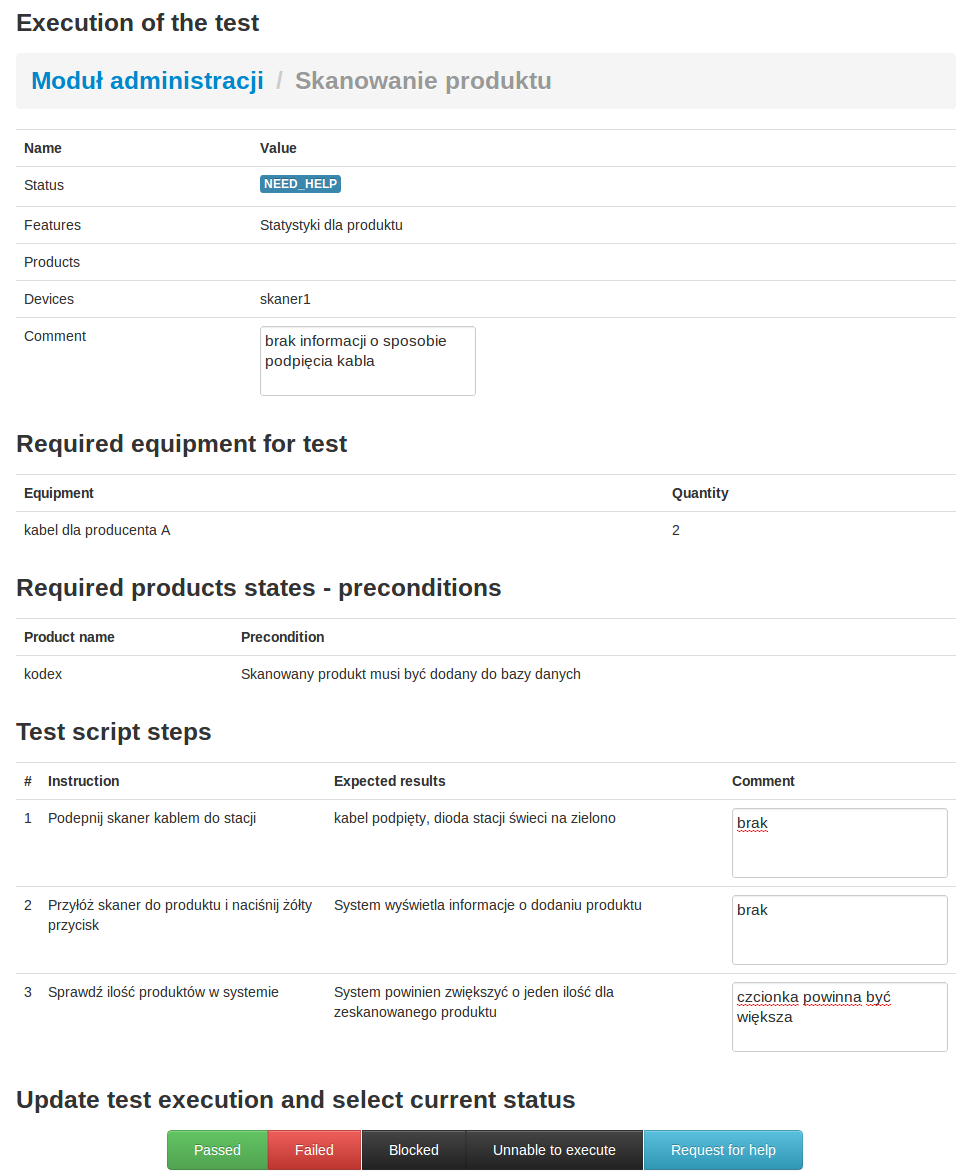
\includegraphics[scale=0.4]{img/screen/wykonanieTestu.png}
    
    \caption{Ekran prezentujący wykonanie testu}
    \label{fig:wykonanieTestu}
  \end{center}
\end{figure}





\section{Scenariusz 4: wykonanie testu z negatywnym rezultatem}

Scenariusz czwarty jest zbliżony do scenariusza trzeciego. Scenariusz ten  zakłada iż użytkownik zmieni stan wykonania testu w taki sposób by końcowy stan testu oznaczał negatywny rezultat. Poprzez negatywny rezultat rozumiemy stan gdy przynajmniej jeden z kroków skryptu testowego wygenerował nieoczekiwany rezultat, warunki początkowe nie mogły zostać spełnione, lub obserwacje innego zachowania systemu wskazują błąd w systemie.

Użytkownik powienien mieć możliwość dokonać następującej ścieżki zmianu statusu testu:

\begin{figure}[h!]
  \begin{center}
   oczekujący $\rightarrow$  przypisany $\rightarrow$ wymagana analiza $\rightarrow$  wynik negatywny
  \end{center}
\end{figure}
\begin{figure}[h!]
  \begin{center}
   oczekujący $\rightarrow$  przypisany $\rightarrow$ zablokowany $\rightarrow$  wynik negatywny
  \end{center}
\end{figure}

\begin{figure}[h!]
  \begin{center}
   oczekujący $\rightarrow$  przypisany $\rightarrow$ wymagana analiza $\rightarrow$  nie możliwy do wykonania
  \end{center}
\end{figure}

Zmiany stanu testu powinny być zachowane w archiwum wykonywanego przypadku testowego jak również powinny zostać wyświetlone na stronie głównej aplikacji. Przejście do stanu końcowego powinno zostać uwzględnione na wykresie spalania testów.

\begin{figure}[h]
\centering
\subfloat[Archiwum dla wykonania testu]{ 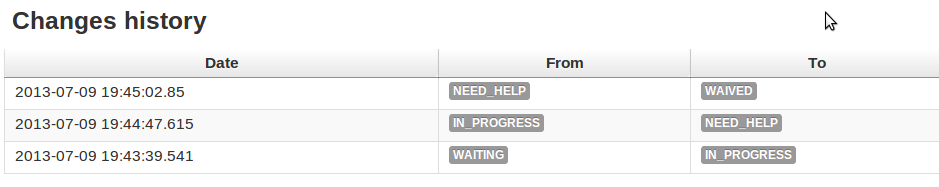
\includegraphics[scale=0.4]{img/screen/zmianyStanuTestu1.png}}\\
\subfloat[Strona główna aplikacji]{ 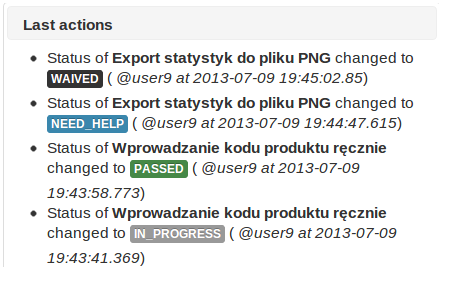
\includegraphics[scale=0.6]{img/screen/zmianyStanuTestu2.png}}

\caption{Prezentacja zmiany stanu testu}
\label{fig:zmianyStanu}
\end{figure}


\section{Scenariusz 5: Analiza wariacji przypadku testowego}

Scenariusz piąty weryfikuje funkcjonalności związane z hurtownią danych aplikacji. Typami funkcjonalności oferowanych przez ten moduł są: dane procentowe prezentujące proporcje dla stanów testów, dane prezentujące postęp wykonania planów testów poprzez wykres spalania, dane ilościowe prezentujące pokrycie funkcjonalności przez testy.

Dodatkową funkcjonalnością jest prezentacja możliwych permutacji dla przypadku testowego. Ta funkcjonalność jest weryfikowana bezpośrednio przez scenariusz piąty. Scenariusz ten zakłada iż osoba administratująca systemem jest w stanie przenalizować możliwe permutacje składowych dla określonego przypadku testowego. System wyświetla informacje na temat permutacji składowych przypadku testowego w postaci grafu skierowanego. W centrum grafu znajduje się przypadek testowy, który połączony jest z wierzchołkami oznaczającymi poszczególny permutacje elementów składowych. Wierzchołki permutacji elementów składowych połączone są z wierzchołkami oznaczającymi permutacje konfiguracji sprzętowej.

Rysunek \ref{fig:permutacje}  prezentuje widok permutacji dla urządzenia, które posiada definicje dwóch grup testowych. Warunki dla poszczególnych elementów definicji testu zostały zdefiniowane w ten sposób iż dla każdej możliwej permutacji urządzeń z dwóch grup generowana jest inna kombinacja dla końcowej definicji testu. Dla każdej z permutacji elementów końcowych możliwe jest wyświetlenie końcowej treści scenariusza.

Analiza danych dostarczana przez grafy permutacji dla przypadków końcowych może być użyta przez koordynatora testów. Na tej podstawie stworzone mogą zostać plany testowe, które na przestrzeni całego wydania systemu testują wszerz możliwe ścieżki przypadków testowych dla systemu.

\begin{figure}[h]
\centering
\subfloat[Permutacja elementów testu]{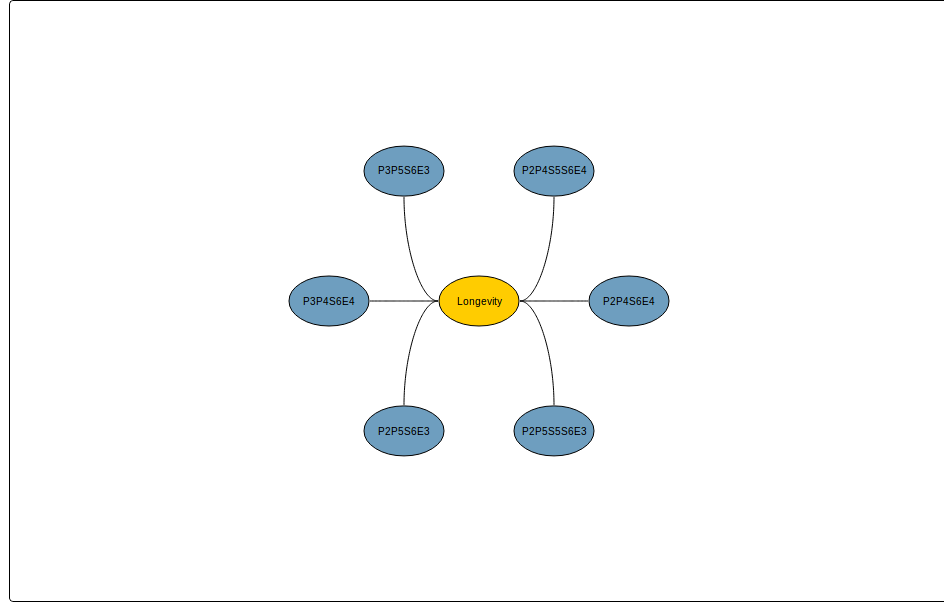
\includegraphics[scale=0.3]{img/screen/PermutacjePrzypadkuTestowego.png}}\qquad
\subfloat[Permutacja urządzeń dla permutacji elementow]{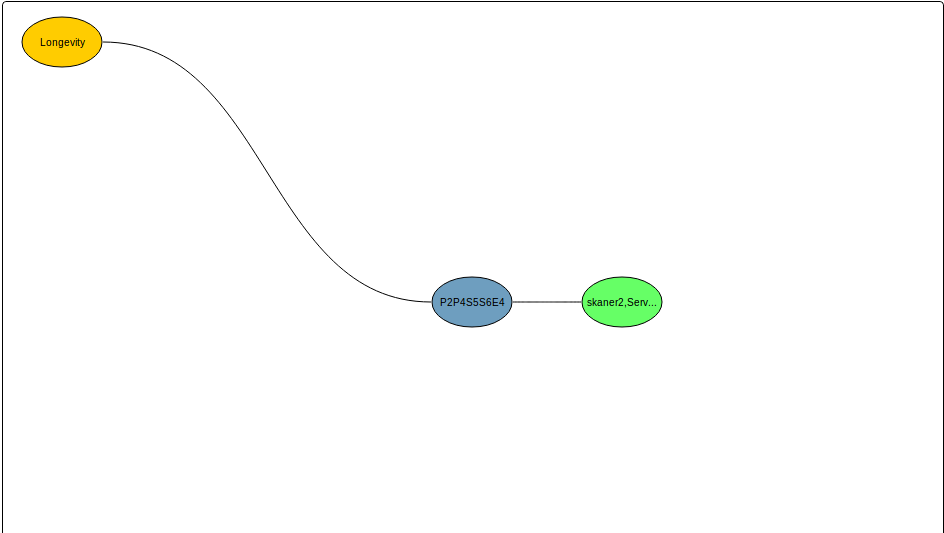
\includegraphics[scale=0.3]{img/screen/konkretnaPermutacja.png}}\\
\subfloat[Detale permutacji elementów]{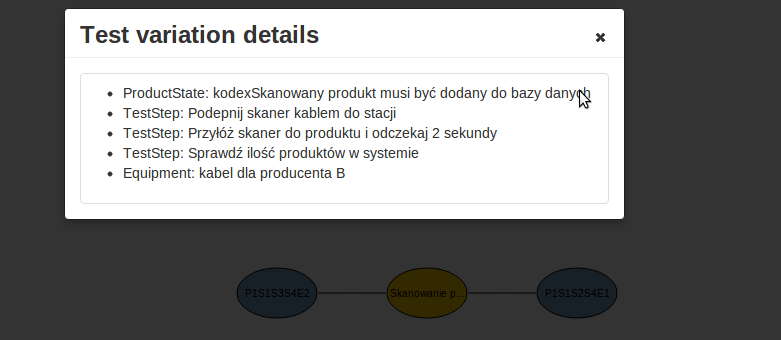
\includegraphics[scale=0.4]{img/screen/permutacjaDetal.png}}%
\caption{Permutacja dla testu.}
\label{fig:permutacje}
\end{figure}

\section{Scenariusz 6: integracja z zewnętrznym oprogramowaniem}

Scenariusz szósty weryfikuje możliwości integracji aplikacji z zewnętrznymi aplikacjami istniejącymi już w systemie. Na potrzeby testowania aplikacji użyto aplikacji \textit{POSTMAN rest client}\cite{postman}, która poprzez interfejs aplikacji internetowej pozwala kierować zapytania typu \textit{REST} do usługi internetowej.

Sprawdzony został możliwy przebieg interakcji komputer-komputer. Założono iż wymaganiem jest możliwość wyświetlania i edycji przypadków testowych dla użytkownika o nazwie \textit{automatyzacja}.

Przypadki testowe dla użytkowika pobierane są poprzez odwołanie się do zasobu konkretnego użytkownika i podzasobu przypadki testowe. Usługa internetowa w zależności od treści nagłówka żądania zwraca odpowiedź w formacie JSON lub XML. Lista przypadków testowych dla użytkownika zawiera odwołania do zasobu oznaczającego poszczególne wykonanie przypadku testowego.

Poprzez odwołanie się do zasobu poszczególnego wykonania przypadku testowego interfejs kliencki komunikujący się z usługą internetową pobiera treść testu do wykonania. Poprzez parsowanie dokumentu XML lub odwołanie się wprost do formatu JSON przez język JavaScript klient wykonuje kroki przypadku testowego. Po zakończonym wykonaniu przypadku testowego, status testu aktualizowany jest poprzez odwołanie się do zasobu poszczególnego wykonania przypadku testowego przy użyciu metody POST.

Aktualizacja przypadku testowego przez usługę internetową wykonuje taki sam przepływ w aplikacji jak wykonanie analogicznej czynności poprzez aplikacje internetową.

\section{Podsumowanie scenariuszy testowych}

Wykonanie przedstawionych scenariuszy testowych przebiegło pomyślnie. Aplikacja spełnia założone wymagania funkcjonalne. Ponadto sprawdzone zostały niefunkcjonalne aspekty aplikacji związane z użytecznością. Ocena użyteczności cechuje się subiektywnością gdyż trudno wydzielić jednoznaczne charakterystyki oceniające poziom użyteczności oprogramowania. Aspektami, które mogą pozytywnie wpływać na użyteczność są: przejrzysty i wyraźny dobór kolorów i czcionek w aplikacji, zastosowania odpowiednich komponentów w formularzach, rozbicie dużych formularzy na mniejsze kroki, zastosowanie funkcjonalności przeciągnij i upuść (ang. \textit{drag and drop}).



\chapter{Zakończenie}

Rozdział siódmy przedstawia możliwe ścieżki rozwoju aplikacji i podsumowuje rezutat otrzymany w trakcie tworzenia niniejszej pracy.

\section{Możliwe ścieżki rozwoju aplikacji}

Stworzona aplikacja nie jest tworem zamkniętym. Może ona zostać rozwinięta o dodatkowe funkcjonalności tak by spełniać dodatkowe wymagania użytkowników. Można wyróżnić dwa aspekty w kierunku, których nastąpić może rozwój aplikacji:
\begin{enumerate}
  \item rozszerzenie ogónych funkcjonalności aplikacji;
  \item rozszerzenie wsparacia integracji z zewnętrznymi aplikacjami.
\end{enumerate}

Przykładowymi funkcjonalnościami, które mogą być dodane do aplikacji są: analiza kosztów testowania i system agentowy służący do pobierania danych pochodzących z wykonania testu.

Poprzez analize kosztów testowania autor rozumie możliwość przypisania określonych kosztów dla poszczególnych elementów składowych testowania. Elementami takimi może być godzina pracy testera, dostarczenie wymaganego sprzętu, koszt instalacji konfiguracji sprzętowej. Zdefiniowane dane mogą posłużyć do analizy kosztów na poziomie permutacji przypadku testowego lub całego planu testów.

Drugą z możliwych funkcjonalności jest zaprojektowanie i zaimplementowanie systemu agentowego, który zbiera artefakty powstałe podczas wykonania przypadku testowego na bieżącym oprogramowaniu i urządzeniach. Agenty te działały by na urządzeniach, na których zainstalowane są produkty poddane testom. Podczas rozpoczęcia przypadku testowego, system przesyła informacje o rozpoczęciu testu do wszystkich agentów, które znajdują się na komputerach, na których znajduje się oprogramowanie, które wymagane jest do wykonania aktualnego przypadku testowego. W przypadku gdy wynik wykonania przypadku testowego byłby negatywny, system automatycznie pobiera poprzez agenty artefakty, które zostaną dołączone do opisu wykonania przypadku testowego. Artefaktami mogą być: logi aplikacji, stan obciążenia procesora i pamięci. Informacje te mogą być przydatne podczas analizy defektu przez zespół programistyczny.

Drugim kierunkiem rozwoju dla aplikacji jest dodanie dostępu do większej liczby funkcjonalności dla interakcji komputer-komputer. Dobór, które funkcjonalności powinny być również udostępnione przez usługę internetową może zostać dokonany podczas normalnego użytkowania aplikacji. Użytkowanie pozwoli wyodrębnić obszary, które mogą zostać zautomatyzowane. Drugim kryterium doboru elementów dla usługi internetowej mogą być wymaganie wynikające wprost z aktualnego stanu oprogramowania wspierającego proces testowania u użytkowika aplikacji. Pozostałe aplikacje użytkowika mogą przechowywać dane, które w sposób automatyczny powinny zostać przeniesione do repozytorium.



\section{Podsumowanie}

Wynikiem niniejszej pracy magisterkiej jest aplikacja będąca repozytorium testów manualnych. Założeniami było spełnienie specyficznych wymagań dla systemów wielowydaniowych, które dedykowane są na wiele urządzeń. Spełnienie przyjętych założeń walidowane było w rozdziale szóstym, który przedstawia możliwe scenariusze procesu testowania oprogramowania względem aplikacji repozytorium.

Specyfika systemów, dla których dedykowane jest repozytorium wymaga odpowiedniego doboru testów gdyż końcowa ilość przypadków testowych składa się z macierzy istniejąych przypadków testowych i permutacji końcowych konfiguracji sprzętowych. Ważnym założeniem aplikacji było umożliwienie jak najprostszego sposobu definicji przypadków testowych, których końcowa treść uzależniona jest od końcowej konfiguracji. Efekt ten udało się osiągnąć poprzez udostępnienie możliwości definiowania warunków dla składowych definicji testów. Drugi aspekt systemów czyli inkrementacyjny sposób tworzenia oprogramowania wspierany jest podczas definicji planów testowych, których specyfikacja wymaga podania wersji oprogramowania. Wersja oprogramowania odpowiada inkrementacji w obrębie jednego wydania.

Aplikacjia udostępnia podstawowe funkcjonalności wymagane do zarządzania przypadkami testowymi, planami testów  i do  wykonywania i raportowania stanu przypadków testowych. Dodatkowo aplikacja udostępnia narzędzia analityczne poprzez hurtownie danych takie jak: wykres spalania testów dla planu testów, wykresy pokrycia funkcjonalności, informacje o zdarzeniach w systemie i grafy permutacji końcowej treści przypadku testowego w zależności od konfiguracji sprzętowej.

Założeniem aplikacji było też umożliwienie integracji z zewnętrznumi aplikacjami. Wymóg ten jest kluczowy ponieważ przedsiębiorstwa na podstawie integracji pojednyńczych aplikacji konstruują złożone systemy testowe. Udało się spełnić to wymaganie poprzez udostępnienie poprzez usługę internetową kluczowych funkcjonalności z perspektywy integracji.

 
